\section{Volume by Cross-Sectional Area; Disk and Washer Methods}\label{sec:disk}

The volume of a general right cylinder, as shown in Figure \ref{fig:cross1}, is 

\hfill Area of the base $\times$ height. \hfill\null

\mtable{.8}{The volume of a general right cylinder}{fig:cross1}{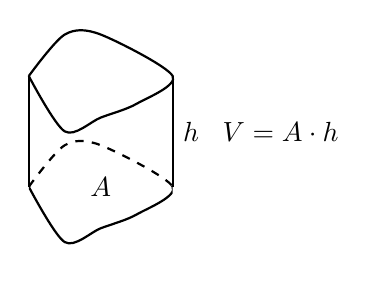
\begin{tikzpicture}[x=13pt,y=10pt,thick]
			\begin{scope}
			\clip (0,0) rectangle (4,-2.5);
			\draw [smooth] plot coordinates {(0,0) (1,1.5) (2,1.5) (4,0) (3,-1) (2,-1.5) (1,-2) (0,0)};
			\end{scope}
			\begin{scope}
			\clip (0,0) rectangle (4,2.5);
			\draw [smooth,dashed] plot coordinates {(0,0) (1,1.5) (2,1.5) (4,0) (3,-1) (2,-1.5) (1,-2) (0,0)};
			\end{scope}
			\begin{scope}[shift={(0,4)}]
			\draw (7,-2) node {$V=A\cdot h$};
			\draw [smooth] plot coordinates {(0,0) (1,1.5) (2,1.5) (4,0) (3,-1) (2,-1.5) (1,-2) (0,0)};
			\end{scope}
			\draw (0,0) -- (0,4) (4,0) -- (4,4) node [pos=.5,right] {$h$};
			\draw (2,0) node {$A$};
			\end{tikzpicture}}

\noindent We can use this fact as the building block in finding volumes of a variety of shapes.

Given an arbitrary solid, we can \textit{approximate} its volume by cutting it into $n$  thin slices. When the slices are thin, each slice can be approximated well by a general right cylinder. Thus the volume of each slice is approximately its cross-sectional area $\times$ thickness. (These slices are the differential elements.)

By orienting a solid along the $x$-axis, we can let $A(x_i)$ represent the cross-sectional area
of the $i\,^\text{th}$ slice, and let $\dx_i$ represent the thickness of this slice (the thickness is a small change in $x$). The total volume of the solid is approximately:
	\begin{align*} \text{Volume} &\approx \sum_{i=1}^n \Big[\text{Area}\ \times\ \text{thickness}\Big] \\
			&= \sum_{i=1}^n A(x_i)\dx_i.
	\end{align*}
	
Recognize that this is a Riemann Sum. By taking a limit (as the thickness of the slices goes to 0) we can find the volume exactly. 

\theorem{thm:volume_by_cross_section}{Volume By Cross-Sectional Area}
{The volume $V$ of a solid, oriented along the $x$-axis with cross-sectional area $A(x)$ from $x=a$ to $x=b$, is \index{integration!volume!cross-sectional area}
$$V = \int_a^b A(x)\ dx.$$
}

\example{ex_disk0}{Finding the volume of a solid}{
Find the volume of a pyramid with a square base of side length 10 in and a height of 5 in.}
{There are many ways to ``orient'' the pyramid along the $x$-axis; Figure \ref{fig:disk0} gives one such way, with the pointed top of the pyramid at the origin and the $x$-axis going through the center of the base.
\mfigure{.35}{Orienting a pyramid along the $x$-axis in Example \ref{ex_disk0}.}{fig:disk0}{figures/figcross_area1}

Each cross section of the pyramid is a square; this is a sample differential element. To determine its area $A(x)$, we need to determine the side lengths of the square.

When $x=5$, the square has side length 10; when $x=0$, the square has side length 0. Since the edges of the pyramid are lines, it is easy to figure that each cross-sectional square has side length $2x$, giving $A(x) = (2x)^2=4x^2$. Following Theorem \ref{thm:volume_by_cross_section}, we have 
\begin{align*} V &= \int_0^5 4x^2\ dx\\
				&= \frac43x^3\Big|_0^5 \\
				&=\frac{500}{3}\ \text{in}^3 \approx 166.67\ \text{in}^3.
\end{align*}
We can check our work by consulting the general equation for the volume of a pyramid (see the back cover under ``Volume of A General Cone''): 

\hfill $\frac13\times \text{area of base}\times \text{height}$.\hfill \null

\noindent Certainly, using this formula from geometry is faster than our new method, but the calculus-based method can be applied to much more than just cones.
}\\

An important special case of Theorem \ref{thm:volume_by_cross_section} is when the solid is a \textbf{solid of revolution}, that is, when the solid is formed by rotating a shape around an axis.

Start with a function $y=f(x)$ from $x=a$ to $x=b$. Revolving this curve about a horizontal axis creates a three-dimensional solid whose cross sections are disks (thin circles). Let $R(x)$ represent the radius of the cross-sectional disk at $x$; the area of this disk is $\pi R(x)^2$. Applying Theorem \ref{thm:volume_by_cross_section} gives the Disk Method.

\keyidea{idea:disk_method}{The Disk Method}
{Let a solid be formed by revolving the curve $y=f(x)$ from $x=a$ to $x=b$ around a horizontal axis, and let $R(x)$ be the radius of the cross-sectional disk at $x$. The volume of the solid is
\index{integration!volume!Disk Method}\index{Disk Method}
$$V = \pi \int_a^b R(x)^2\ dx.$$
}

\example{ex_disk1}{Finding volume using the Disk Method}{
Find the volume of the solid formed by revolving the curve $y=1/x$, from $x=1$ to $x=2$, around the $x$-axis.}
{A sketch can help us understand this problem. In Figure \ref{fig:disk1} (a) the curve $y=1/x$ is sketched along with the differential element -- a disk -- at $x$ with radius $R(x)=1/x$. In Figure \ref{fig:disk1} (b) the whole solid is pictured, along with the differential element. 

Using Key Idea \ref{idea:disk_method}, we have 
\begin{align*}
	V &= \pi\int_1^2 \left(\frac1x\right)^2\ dx \\
		&= \pi\int_1^2 \frac1{x^2}\ dx \\
		&= \pi\left[-\frac1x\right]\Big|_1^2 \\
		&= \pi \left[-\frac12 - \left(-1\right)\right] \\
		&= \frac{\pi}{2}\ \text{units}^3.
\end{align*}
\mtable{.75}{Sketching a solid in Example \ref{ex_disk1}.}{fig:disk1}{%
		\begin{tabular}{c} %
		\myincludegraphics{figures/figdisk1} \\
		(a) \\
		\myincludegraphics{figures/figdisk1b} \\
		(b) 
		\end{tabular}
}
\vskip-\baselineskip
}\\

While Key Idea \ref{idea:disk_method} is given in terms of functions of $x$, the principle involved can be applied to functions of $y$ when the axis of rotation is vertical, not horizontal. We demonstrate this in the next example.\\

\example{ex_disk2}{Finding volume using the Disk Method}{
Find the volume of the solid formed by revolving the curve $y=1/x$, from $x=1$ to $x=2$, about the $y$-axis.}
{Since the axis of rotation is vertical, we need to convert the function into a function of $y$ and convert the $x$-bounds to $y$-bounds. Since $y=1/x$ defines the curve, we rewrite it as $x=1/y$. The bound $x=1$ corresponds to the $y$-bound $y=1$, and the bound $x=2$ corresponds to the $y$-bound $y=1/2$. 

Thus we are rotating the curve $x=1/y$, from $y=1/2$ to $y=1$ about the $y$-axis to form a solid. The curve and sample differential element are sketched in Figure \ref{fig:disk2} (a), with a full sketch of the solid in Figure \ref{fig:disk2} (b).
\mtable{.4}{Sketching the solid in Example \ref{ex_disk2}.}{fig:disk2}{%
		\begin{tabular}{c}
		\myincludegraphics{figures/figdisk1a} \\
		(a)\\
		\myincludegraphics{figures/figdisk2a} \\
		(b)
		\end{tabular}
		}
We integrate to find the volume:
\begin{align*}
V &= \pi\int_{1/2}^1 \frac{1}{y^2}\ dy \\
	&= -\frac{\pi}y\Big|_{1/2}^1 \\
	&= \pi\ \text{units}^3.
\end{align*}		
}\\

We can also compute the volume of solids of revolution that have a hole in the center. The general principle is simple: compute the volume of the solid irrespective of the hole, then subtract the volume of the hole. If the outside radius of the solid is $R(x)$ and the inside radius (defining the hole) is $r(x)$, then the volume is 
$$V = \pi\int_a^b R(x)^2 \ dx - \pi\int_a^b r(x)^2\ dx = \pi\int_a^b \left(R(x)^2-r(x)^2\right)\ dx.$$

One can generate a solid of revolution with a hole in the middle by revolving a region about an axis. Consider Figure \ref{fig:washeridea} (a), where a region is sketched along with a dashed, horizontal axis of rotation. By rotating the region about the axis, a solid is formed as sketched in Figure \ref{fig:washeridea} (b). The outside of the solid has radius $R(x)$, whereas the inside has radius $r(x)$. Each cross section of this solid will be a washer (a disk with a hole in the center) as sketched in Figure \ref{fig:washeridea} (c).	This leads us to the Washer Method.
\mtable{.67}{Establishing the Washer Method.}{fig:washeridea}{%
\begin{tabular}{c}
\myincludegraphics{figures/figwasher_idea_a}\\
(a) \\
\myincludegraphics{figures/figwasher_idea_b}\\
(b) \\
\myincludegraphics{figures/figwasher_idea_c}\\
(c)
\end{tabular}
}

\keyidea{idea:washermethod}{The Washer Method}
{Let a region bounded by $y=f(x)$, $y=g(x)$, $x=a$ and $x=b$ be rotated about a horizontal axis that does not intersect the region, forming a solid. Each cross section at $x$ will be a washer with outside radius $R(x)$ and inside radius $r(x)$. The volume of the solid is
\index{integration!volume!Washer Method}\index{Washer Method}
$$V = \pi\int_a^b \Big(R(x)^2-r(x)^2\Big)\ dx.$$ 
}

Even though we introduced it first, the Disk Method is just a special case of the Washer Method with an inside radius of $r(x)=0$.		\\

\example{ex_wash1}{Finding volume with the Washer Method}{
Find the volume of the solid formed by rotating the region bounded by $y=x^2-2x+2$ and $y=2x-1$ about the $x$-axis.}
{A sketch of the region will help, as given in Figure \ref{fig:wash1a}.
\mfigure{.29}{A sketch of the region used in Example \ref{ex_wash1}.}{fig:wash1a}{figures/figwash1} Rotating about the $x$-axis will produce cross sections in the shape of washers, as shown in Figure \ref{fig:wash1} (a); the complete solid is shown in part (b). The outside radius of this washer is $R(x) = 2x+1$; the inside radius is $r(x) = x^2-2x+4$. As the region is bounded from $x=1$ to $x=3$, we integrate as follows to compute the volume.
\begin{align*}
V &= \pi\int_1^3 \Big((2x-1)^2-(x^2-2x+2)^2\Big)\ dx \\
		&= \pi\int_1^3 \big(-x^4+4x^3-4x^2+4x-3\big)\ dx \\
		&= \pi\Big[-\frac{1}{5}x^5+x^4-\frac43x^3+2x^2-3x\Big]\Big|_1^3 \\
		&=\frac{104}{15}\pi \approx 21.78\ \text{units}^3.
\end{align*}	
\vskip-\baselineskip	
\mtable{.76}{Sketching the differential element and solid in Example \ref{ex_wash1}.}{fig:wash1}{%
\begin{tabular}{c}
\myincludegraphics{figures/figwash1c}\\
(a)\\
\myincludegraphics{figures/figwash1b}\\
(b)
\end{tabular}
}

}\\	

When rotating about a vertical axis, the outside and inside radius functions must be functions of $y$.\\

\example{ex_wash2}{Finding volume with the Washer Method}{
Find the volume of the solid formed by rotating the triangular region with vertices at $(1,1)$, $(2,1)$ and $(2,3)$ about the $y$-axis.}
{The triangular region is sketched in Figure \ref{fig:wash2} (a); the differential element is sketched in (b) and the full solid is drawn in (c). They help us establish the outside and inside radii. Since the axis of rotation is vertical, each radius is a function of $y$. 

The outside radius $R(y)$ is formed by the line connecting $(2,1)$ and $(2,3)$; it is a constant function, as regardless of the $y$-value the distance from the line to the axis of rotation is 2. Thus $R(y)=2$. 
\mtable{.32}{Sketching the solid in Example \ref{ex_wash2}.}{fig:wash2}{%
\begin{tabular}{c}
\myincludegraphics{figures/figwash2a} \\
(a) \\
\myincludegraphics{figures/figwash2b} \\
(b) \\
\myincludegraphics{figures/figwash2c} \\
(c)
\end{tabular}
}

The inside radius is formed by the line connecting $(1,1)$ and $(2,3)$. The equation of this line is $y=2x-1$, but we need to refer to it as a function of $y$. Solving for $x$ gives $r(y) = \frac12(y+1)$. 

We integrate over the $y$-bounds of $y=1$ to $y=3$. Thus the volume is
\begin{align*}
V 	&=	\pi\int_1^3\Big(2^2 - \big(\frac12(y+1)\big)^2\Big)\ dy \\
		&=	\pi\int_1^3\Big(-\frac14y^2-\frac12y+\frac{15}4\Big)\ dy \\
		&= 	\pi\Big[-\frac1{12}y^3-\frac14y^2+\frac{15}4y\Big]\Big|_1^3\\
		&= \frac{10}3\pi \approx 10.47\ \text{units}^3.
\end{align*}
\vskip-\baselineskip
}

\printexercises{exercises/07_02_exercises}